\documentclass[conference]{IEEEtran}

\usepackage[T1]{fontenc}
\usepackage[utf8]{inputenc}
\usepackage{graphicx}
\usepackage{booktabs}
\usepackage{cite}
\usepackage{xcolor}
\usepackage{listings}
\usepackage{balance}
\usepackage{float}
\usepackage[hidelinks]{hyperref}

\newcommand{\secref}[1]{\hyperref[#1]{Section~\ref*{#1}}}
\newcommand{\tabref}[1]{\hyperref[#1]{Table~\ref*{#1}}}
\newcommand{\figref}[1]{\hyperref[#1]{Figure~\ref*{#1}}}
\newcommand{\lstrefx}[1]{\hyperref[#1]{Listing~\ref*{#1}}}

\lstdefinestyle{pythonstyle}{
    language=Python,
    basicstyle=\ttfamily\scriptsize,
    keywordstyle=\color{blue!70!black},
    commentstyle=\color{green!40!black},
    stringstyle=\color{orange!60!black},
    showstringspaces=false,
    breaklines=true,
    frame=single,
    tabsize=4
}

\title{From-Scratch CNN Classification, Pure-Noise GAN Augmentation, and CycleGAN Style Transfer for a Cow-Horse Dataset}

\author{\IEEEauthorblockN{Qifeng LIU}}

\begin{document}
\maketitle

\begin{abstract}
In this report, I address three tasks on a cow-horse dataset: image classification, GAN-based data augmentation, and unpaired style transfer. I train a compact convolutional neural network from scratch and stabilize it with a horse-sensitive cross-entropy loss and a three-seed ensemble. I then train class-specific pure-noise GANs, export valid synthetic candidates, and manually curate the final augmentation subset. The best improvement comes from asymmetric manual augmentation of the weaker horse class, where 12 selected synthetic horses increase the final classification accuracy from 65.85\% to 67.07\%. Finally, I report qualitative CycleGAN-style translations between cows and horses.
\end{abstract}

\section{Introduction}\label{sec:intro}
This project contains three connected tasks: a CNN classifier, GAN-based data augmentation, and unpaired neural style transfer. The dataset is challenging because the training split contains only one cow instance and one horse instance observed from multiple viewpoints, while the test split contains unseen instances under the same viewpoint grid. As a result, the main risk is not class imbalance in the dataset itself, but unstable generalization from one instance to another.

My final conclusion is that a compact from-scratch CNN, combined with targeted horse-sensitive training choices, works better than heavier or more symmetric alternatives. In particular, Task 2 improves only after the final augmentation subset is manually curated and applied asymmetrically to the weaker horse class. The rest of the report is organized as follows: \secref{sec:data} introduces the dataset and evaluation protocol, \secref{sec:task1}--\secref{sec:task3} present the three tasks, and \secref{sec:conclusion} summarizes the main takeaways.

\section{Dataset and Evaluation Protocol}\label{sec:data}
The dataset contains 82 training images and 82 test images, with 41 cows and 41 horses in each split. Because the two classes are balanced, overall accuracy and balanced accuracy are numerically identical. However, class-wise accuracy remains essential because the main practical difficulty is that horse recognition is weaker than cow recognition.

\begin{table}[H]
\centering
\caption{Dataset split summary.}
\label{tab:dataset}
\begin{tabular}{lcc}
\toprule
Split & Cow & Horse \\
\midrule
Train & 41 & 41 \\
Test & 41 & 41 \\
\bottomrule
\end{tabular}

\end{table}

\tabref{tab:dataset} summarizes the split that is used consistently in the three tasks.

\section{Task 1: CNN Classification}\label{sec:task1}
\subsection{Preprocessing and training strategy}
I keep preprocessing light and label-preserving: resizing, horizontal flipping, and small rotations. This is appropriate because the dataset is tiny, and stronger augmentation could distort the animal shape more than it helps. During training, inverse-class-frequency sampling balances the classes, alongside a class-weighted cross-entropy loss. The loss weight ratio is set to \([1, 5]\) for cow and horse, respectively. This is a central design choice, because the horse class is the weaker class and needs stronger emphasis during optimization.

Each single training run remains unstable on this dataset, so I train the same model with three fixed seeds and average the final logits. This ensemble reduces seed sensitivity without changing the architecture or introducing pretrained components.

\subsection{CNN architecture}
The classifier is intentionally small because overfitting is the main risk. I use three convolutional blocks followed by global average pooling and a compact classification head. Each block follows the pattern \texttt{Conv + BatchNorm + ReLU + MaxPool}. Convolution extracts local visual cues, batch normalization stabilizes intermediate activations, ReLU keeps the representation non-linear, and max-pooling gradually reduces spatial resolution while preserving the strongest local responses.

The first block captures low-level edges and the global silhouette of the animal. The second block combines these primitive cues into more informative local contour and texture patterns. The third block produces higher-level class cues before the final pooling stage. I use global average pooling instead of a large fully connected stack because it drastically reduces the number of parameters and therefore limits memorization on this very small dataset. The classifier head remains small for the same reason. \lstrefx{lst:cnn} shows the compact architecture used in all Task 1 runs.

\begin{lstlisting}[style=pythonstyle,caption={Compact from-scratch CNN used in Task 1.},label={lst:cnn}]
class SimpleClassifier(nn.Module):
    def __init__(self, num_classes=2):
        super().__init__()
        self.block1 = nn.Sequential(
            nn.Conv2d(3, 16, 3, padding=1),
            nn.BatchNorm2d(16), nn.ReLU(inplace=True),
            nn.MaxPool2d(2)
        )
        self.block2 = nn.Sequential(
            nn.Conv2d(16, 32, 3, padding=1),
            nn.BatchNorm2d(32), nn.ReLU(inplace=True),
            nn.MaxPool2d(2)
        )
        self.block3 = nn.Sequential(
            nn.Conv2d(32, 64, 3, padding=1),
            nn.BatchNorm2d(64), nn.ReLU(inplace=True),
            nn.MaxPool2d(2)
        )
        self.global_pool = nn.AdaptiveAvgPool2d((1, 1))
        self.classifier = nn.Sequential(
            nn.Flatten(), nn.Linear(64, 32),
            nn.ReLU(inplace=True), nn.Dropout(0.25),
            nn.Linear(32, num_classes)
        )
\end{lstlisting}

\subsection{Task 1 results}
\tabref{tab:task1seeds} shows the three seed-specific results together with the final ensemble result. The final Task 1 prediction is not obtained by averaging the three accuracies. Instead, I average the logits produced by the three seed-specific models for each test image and then take the final class decision from the combined logits. With this logit-level ensemble, the final Task 1 performance reaches 65.85\% overall accuracy, with 75.61\% on cows and 56.10\% on horses. \figref{fig:task1overview} complements these numbers by showing both the optimization behavior across seeds and the final confusion matrix. Together, \tabref{tab:task1seeds}, \lstrefx{lst:cnn}, and \figref{fig:task1overview} show that the combination of a compact architecture, class weighting, and ensembling is already sufficient to produce a usable baseline from scratch.

\begin{table}[H]
\centering
\caption{Task 1 seed-wise results and final logit-level ensemble.}
\label{tab:task1seeds}
\begin{tabular}{cccc}
\toprule
Run & Overall & Cow & Horse \\
\midrule
11 & 59.76\% & 70.73\% & 48.78\% \\
21 & 58.54\% & 51.22\% & 65.85\% \\
31 & 58.54\% & 80.49\% & 36.59\% \\
\midrule
Ensemble & 65.85\% & 75.61\% & 56.10\% \\
\bottomrule
\end{tabular}

\end{table}

\begin{figure}[H]
\centering
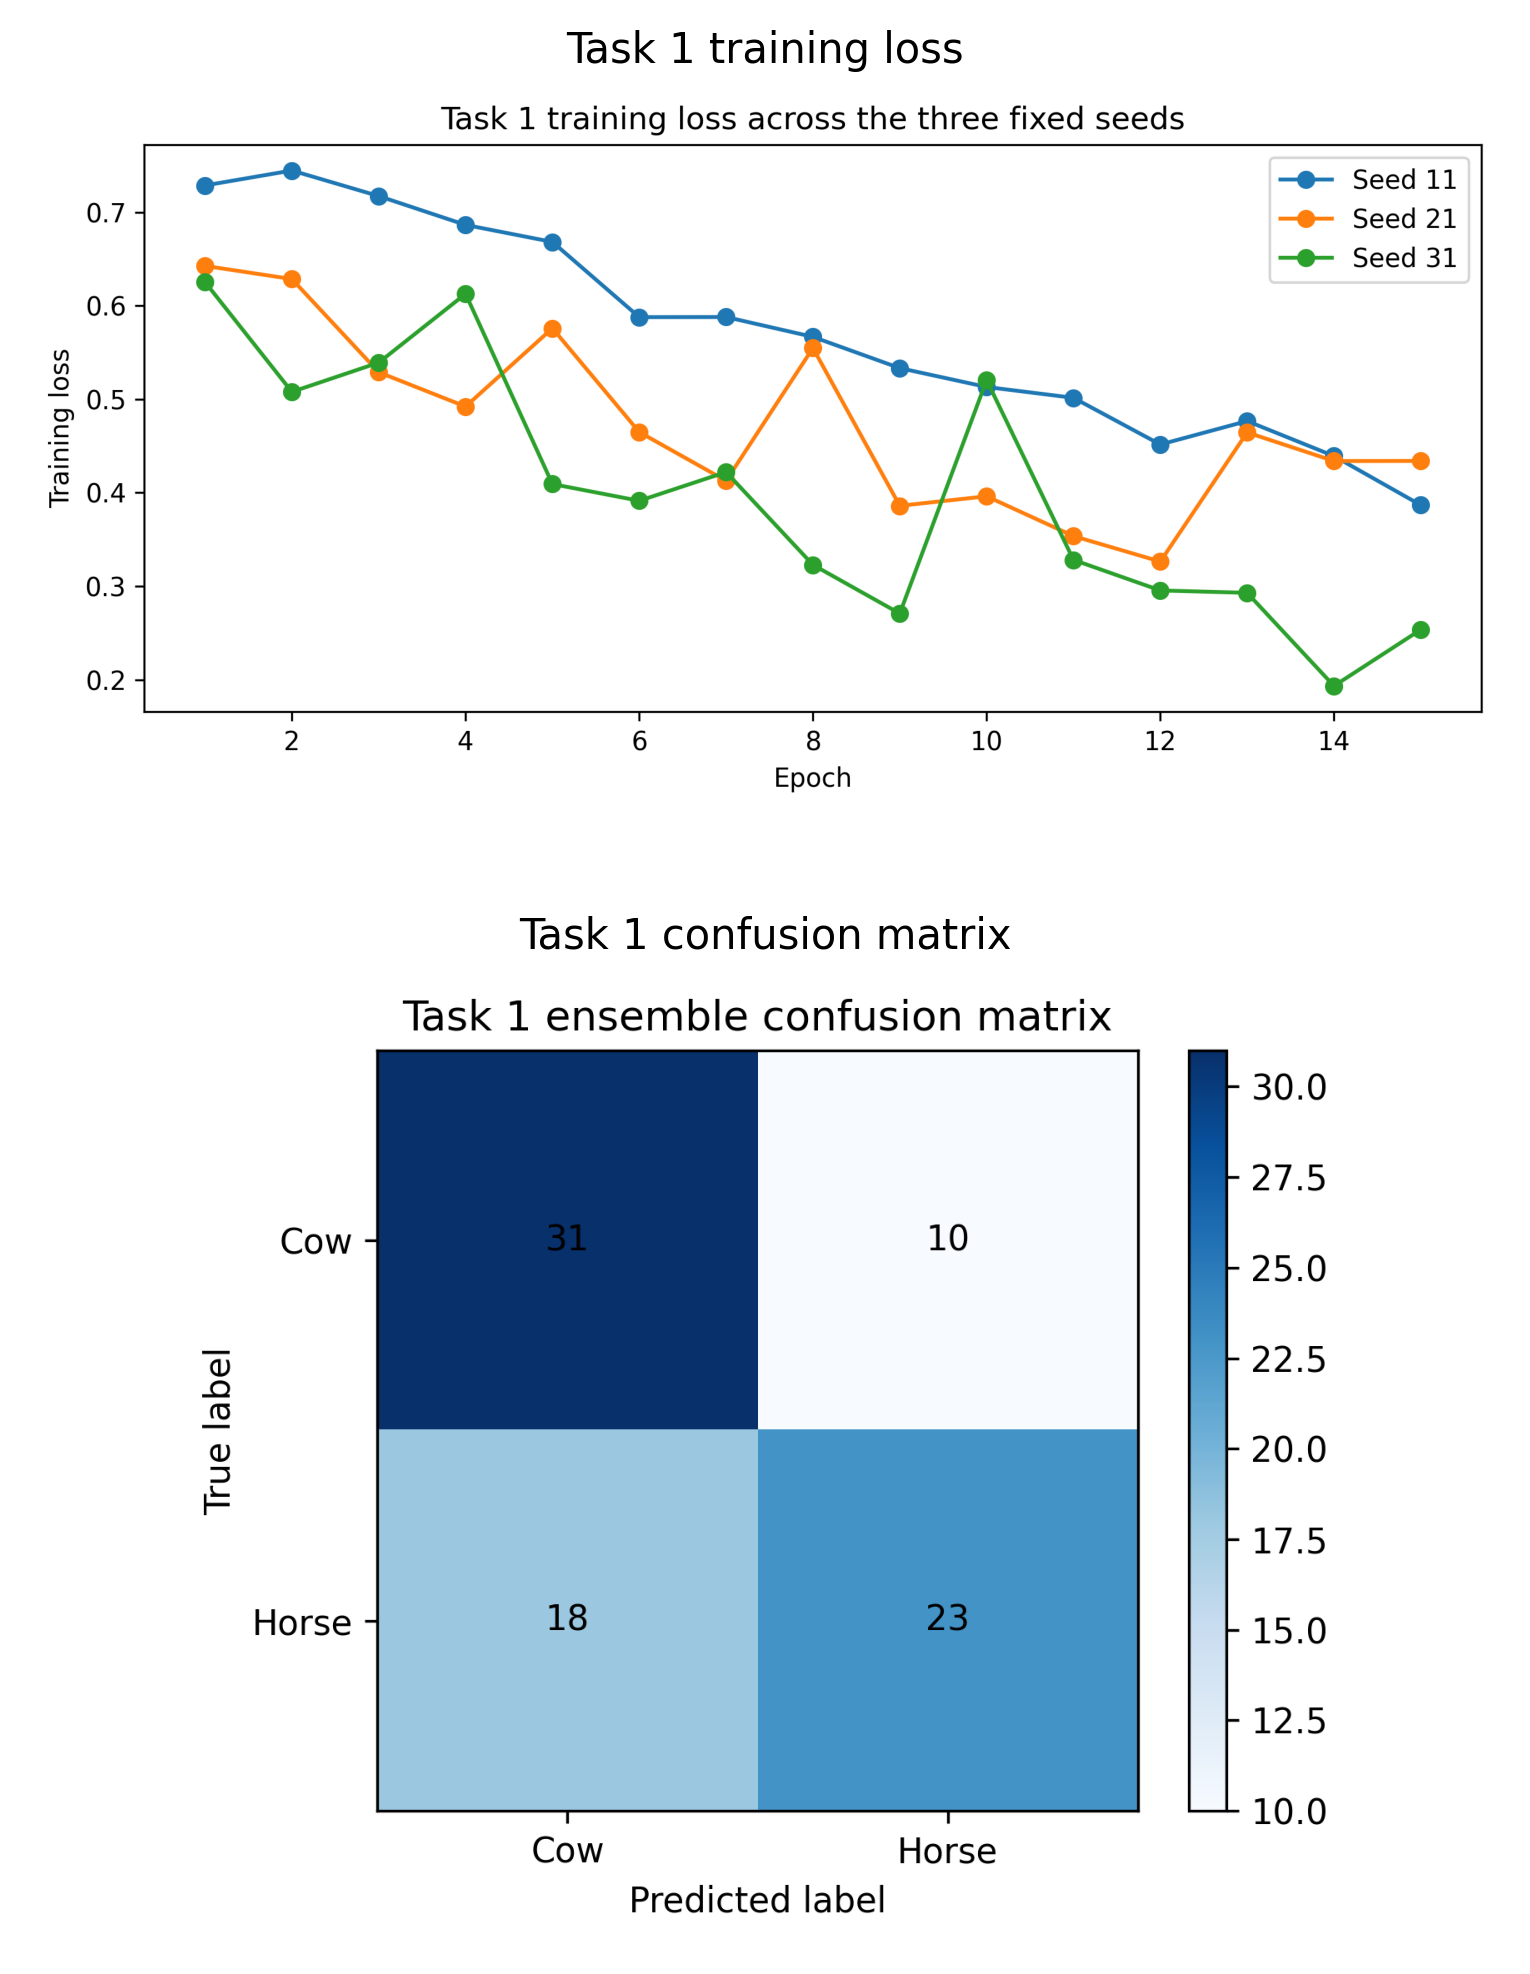
\includegraphics[width=\columnwidth]{generated/figures/task1_overview.png}
\caption{Task 1 overview: training loss across the three fixed seeds and the final ensemble confusion matrix.}
\label{fig:task1overview}
\end{figure}

\section{Task 2: GAN-Based Data Augmentation}\label{sec:task2}
\subsection{GAN design}
Task 2 must start from pure noise, following the original GAN formulation~\cite{goodfellow2014gan}. For this reason, the generator receives only a latent vector of dimension 100 and synthesizes the image from scratch. I train one GAN for cows and one GAN for horses, because the two classes do not behave identically during adversarial training.

The generator first projects the latent vector into a compact spatial tensor and then upsamples it progressively. I use \texttt{Upsample + Conv2d} instead of transpose convolution because this tends to reduce checkerboard artifacts. Batch normalization stabilizes intermediate feature statistics, LeakyReLU keeps gradients flowing in negative activations, and the final \texttt{Tanh} maps the output to the same normalized range used throughout the notebook. The core structure is shown in \lstrefx{lst:task2gan}.

The discriminator uses stride-2 convolutions to reduce spatial resolution progressively and convert the image into higher-level realism cues. I keep it relatively small because the dataset is tiny; an overly strong discriminator quickly memorizes the real images and gives the generator unhelpful gradients.

\begin{lstlisting}[style=pythonstyle,caption={Core Task 2 GAN architecture.},label={lst:task2gan}]
class StableGenerator(nn.Module):
    def __init__(self, latent_dim=100):
        super().__init__()
        self.l1 = nn.Linear(latent_dim, 256 * s * s)
        self.conv_blocks = nn.Sequential(
            conv_block(256, 128), conv_block(128, 64),
            conv_block(64, 32), conv_block(32, 16),
            nn.Conv2d(16, 16, 3, padding=1),
            nn.BatchNorm2d(16), nn.LeakyReLU(0.2, True),
            nn.Conv2d(16, 3, 3, padding=1), nn.Tanh()
        )

class StableDiscriminator(nn.Module):
    def __init__(self):
        super().__init__()
        self.features = nn.Sequential(
            block(3, 16, use_bn=False), block(16, 32),
            block(32, 64), block(64, 128)
        )
        self.classifier = nn.Sequential(
            nn.Flatten(), nn.Linear(128 * s * s, 1), nn.Sigmoid()
        )
\end{lstlisting}

\subsection{Valid-candidate bank}
I do not use every GAN output. Instead, I build a valid-candidate bank from the best checkpoint of each class. Each class-specific GAN is trained for a total of 1000 epochs. Within this training budget, checkpoint selection is performed with a fixed noise bank, evaluated every 50 epochs and previewed every 100 epochs. A candidate is kept only if it passes three automatic conditions: a minimum Task 1 classifier confidence, a minimum discriminator realism score, and a sharpness threshold derived from the real class statistics.

The best valid banks come from epoch 900 for cows and epoch 1000 for horses. At these checkpoints, the exported valid bank contains 34 cow images and 24 horse images. \figref{fig:task2epochs} shows only the 900/1000 previews because they are the most informative late-training checkpoints and visually the strongest among the saved generations.

\begin{figure*}[!t]
\centering
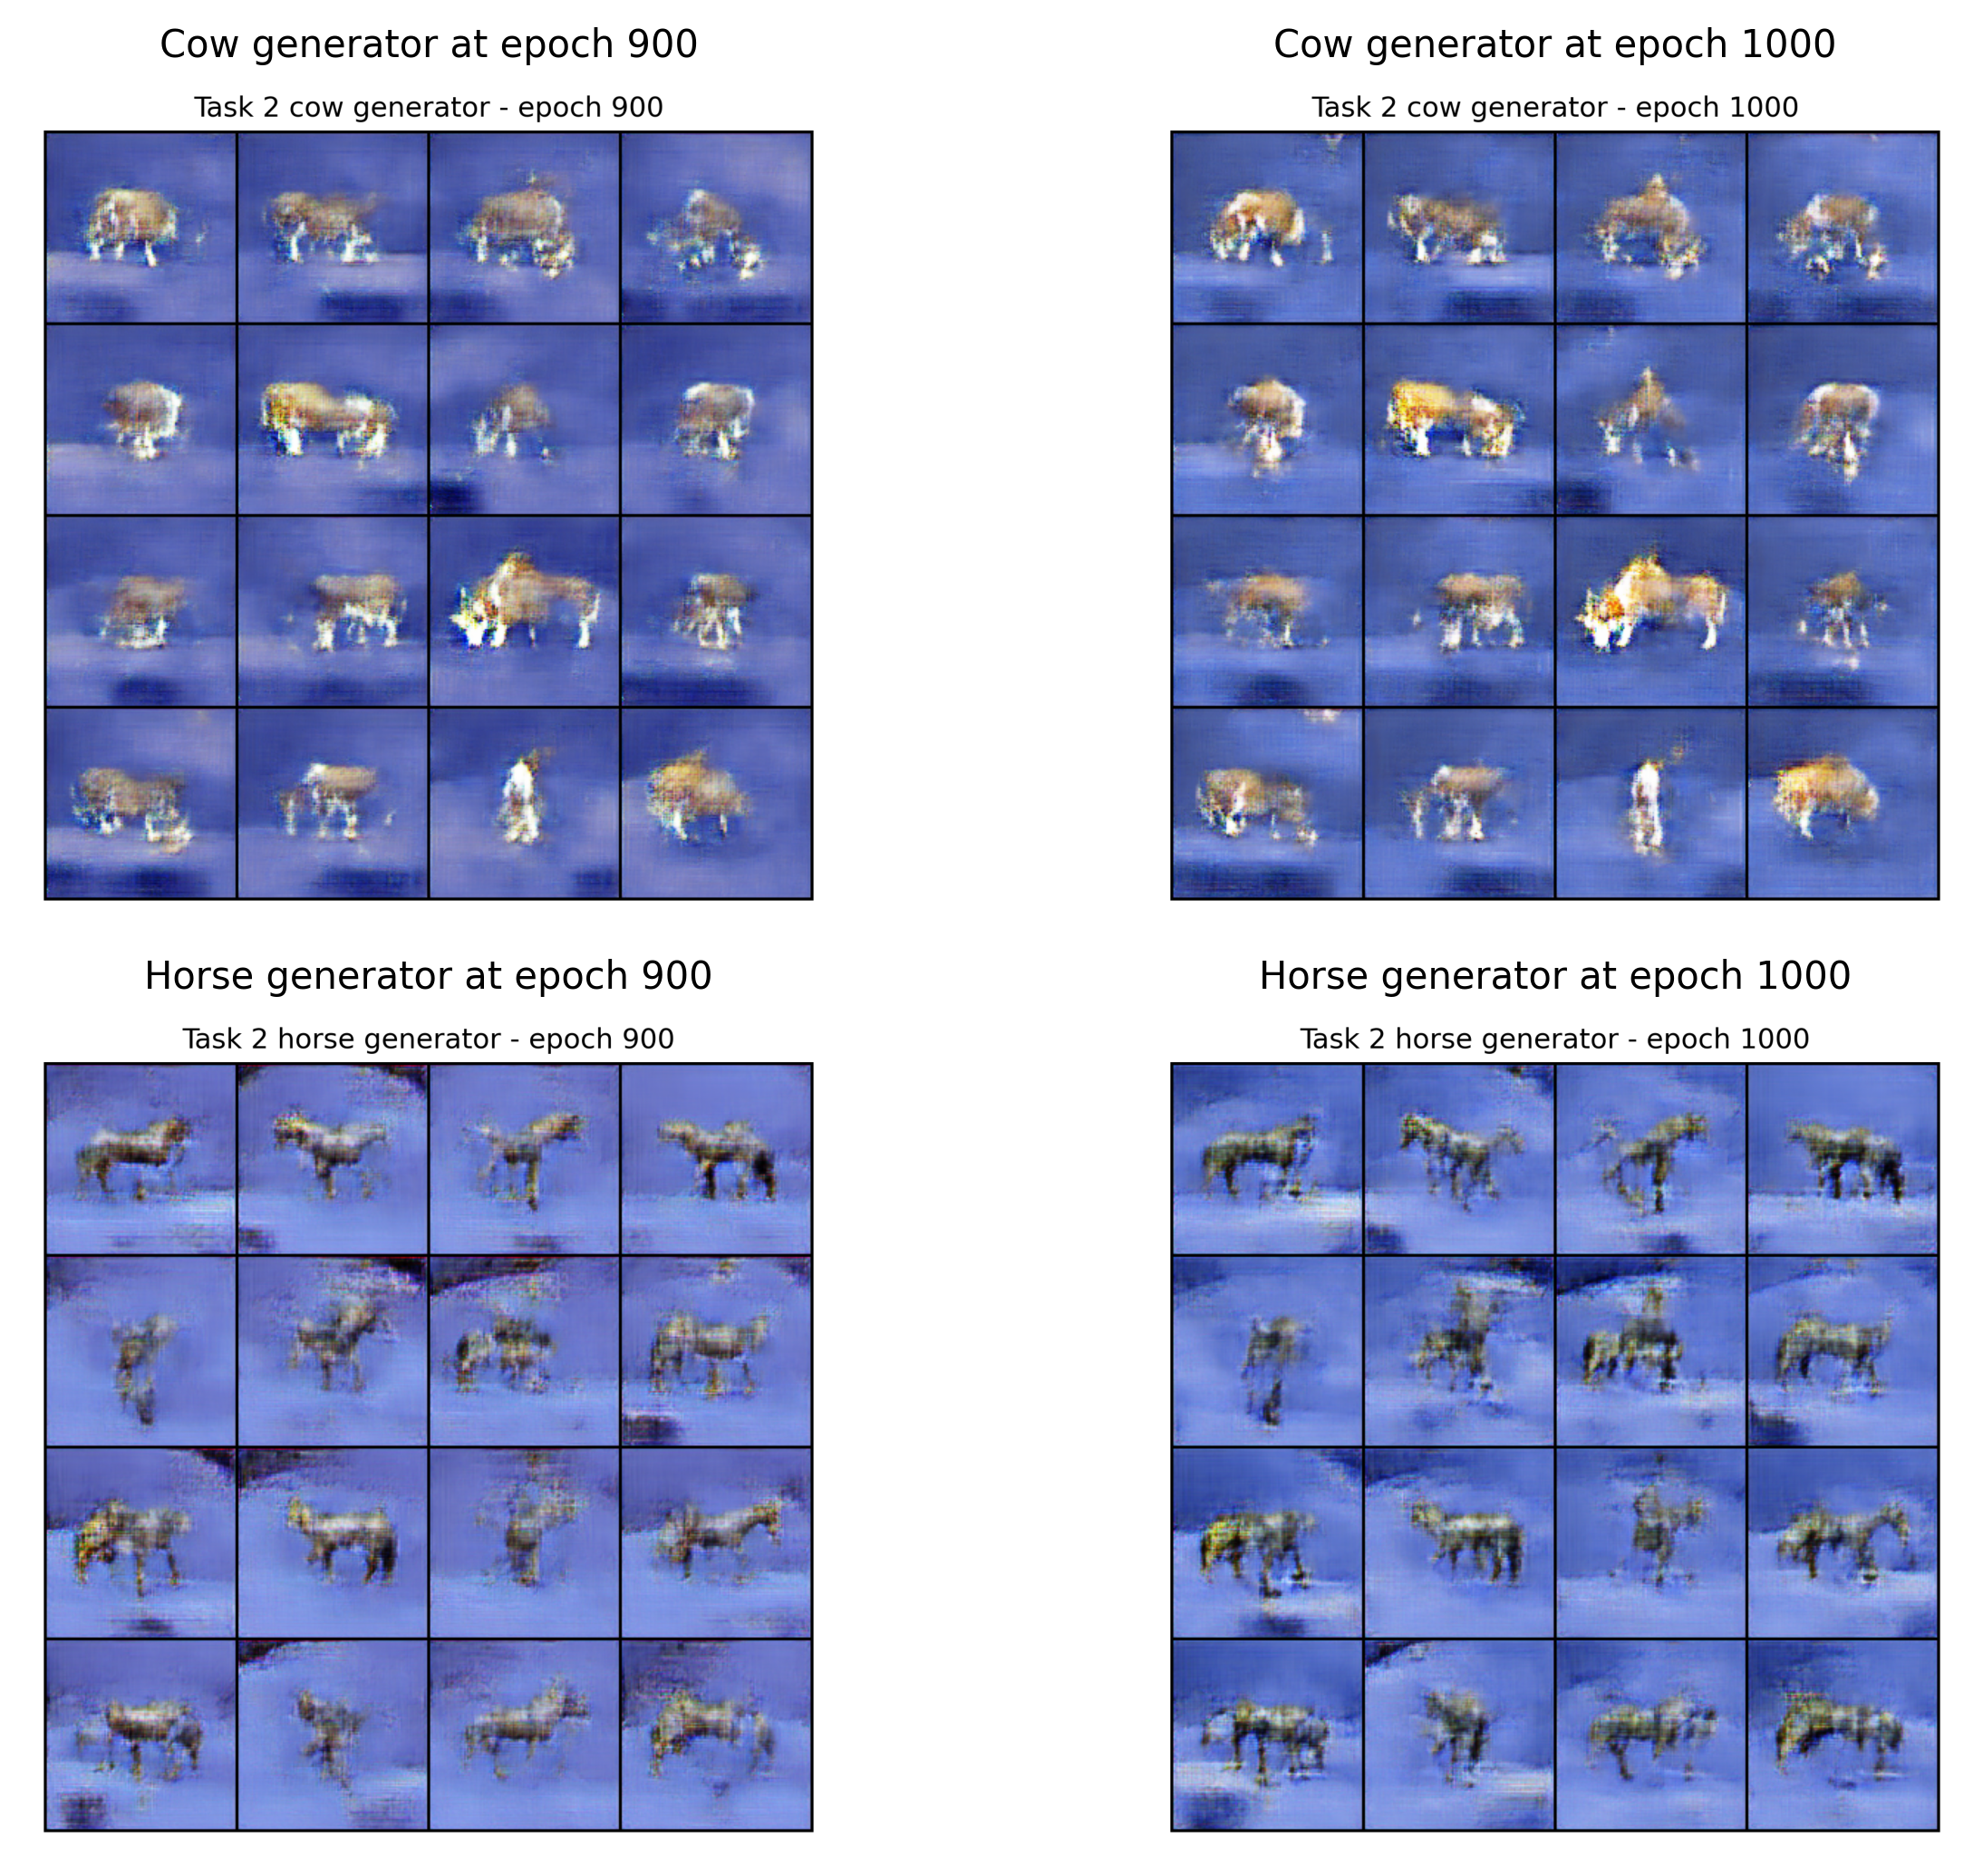
\includegraphics[width=\textwidth]{generated/figures/task2_epoch_grid.png}
\caption{Task 2 GAN previews at the strongest late checkpoints used in the final analysis. The best valid candidate banks come from cow epoch 900 and horse epoch 1000.}
\label{fig:task2epochs}
\end{figure*}

\subsection{Manual asymmetric augmentation}
Automatic scoring is useful for constructing a valid candidate bank, but it is not sufficient for the final augmentation subset. The main reason is that global animal shape is easier to judge visually than with a single scalar score. I therefore manually inspect the valid bank shown in \figref{fig:task2epochs} and move the accepted files into a dedicated \texttt{selected} folder.

The final augmentation is intentionally asymmetric: I keep 0 synthetic cows and 12 synthetic horses. This is justified because cow accuracy is already strong in Task 1, while horse recognition remains the main weakness. Adding more cows tends to reinforce the easier class without improving the weaker one. Once the synthetic horses are manually curated, I set \texttt{synthetic\_sample\_weight = 1.0} so that they have enough influence during retraining. \figref{fig:selectedhorses} summarizes both the final selected horse subset and the failed pretrained-discriminator experiment that motivated the simpler from-scratch discriminator, while \tabref{tab:task1task2} quantifies the final gain.

\begin{figure}[H]
\centering
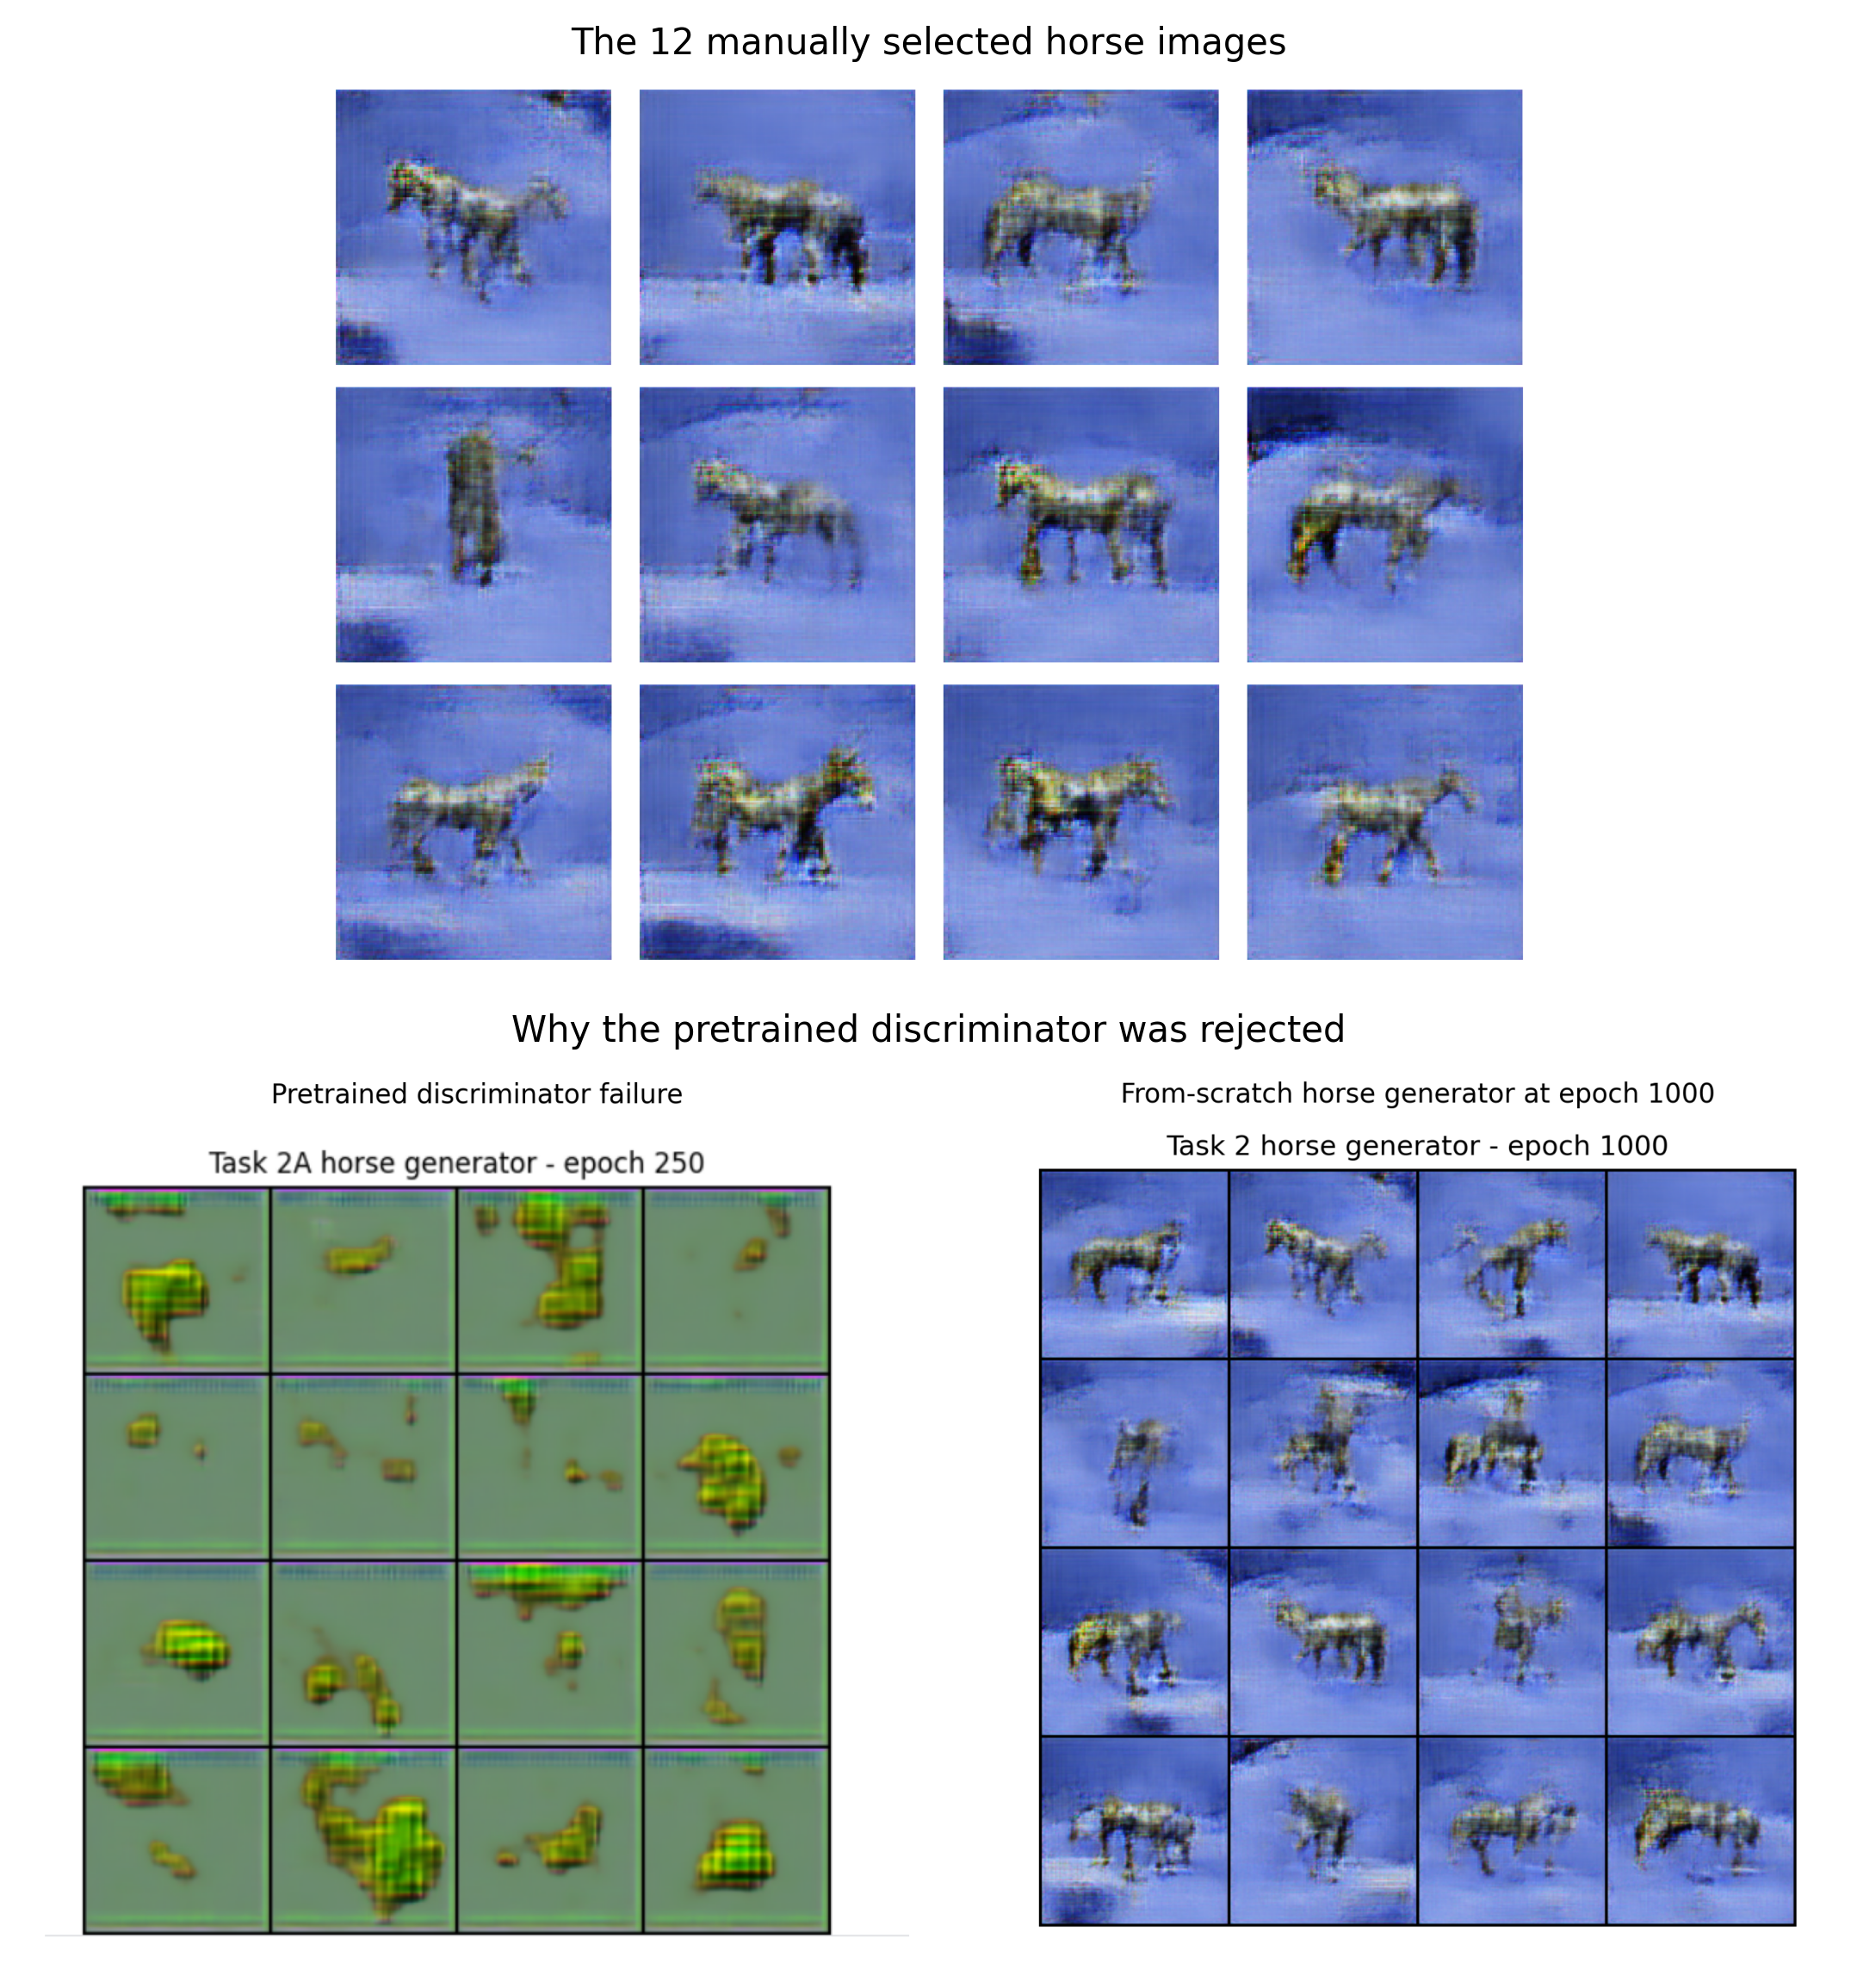
\includegraphics[width=\columnwidth]{generated/figures/task2_manual_overview.png}
\caption{Task 2 manual augmentation evidence. The top panel shows the 12 selected horse images used for retraining. The bottom panel contrasts the failed pretrained-discriminator attempt with the final from-scratch horse generator.}
\label{fig:selectedhorses}
\end{figure}

\begin{table}[H]
\centering
\scriptsize
\caption{Task 1 vs. final Task 2 comparison.}
\label{tab:task1task2}
\begin{tabular}{p{2.1cm}ccccc}
\toprule
Method & Overall & Cow & Horse & Sel. Cow & Sel. Horse \\
\midrule
Task 1 CNN & 65.85\% & 75.61\% & 56.10\% & 0 & 0 \\
Task 2 + 12 horses & 67.07\% & 75.61\% & 58.54\% & 0 & 12 \\
\bottomrule
\end{tabular}

\end{table}

The final Task 2 result reaches 67.07\% overall accuracy, with cow accuracy unchanged at 75.61\% and horse accuracy improved from 56.10\% to 58.54\%. Therefore, the gain comes from the weaker horse class only. \tabref{tab:task1task2} makes this asymmetric effect explicit. The main lesson is that the improvement is driven by targeted asymmetric augmentation of the weaker class, not by generic balanced augmentation.

\section{Task 3: Unpaired Style Transfer}\label{sec:task3}
For Task 3, I implement an unpaired CycleGAN-style system~\cite{zhu2017cyclegan}. The generators use residual blocks so that the model can transform appearance while preserving the main content pathway. In practice, the generator first maps the image into a learned feature space, applies several residual transformations at the bottleneck, and then reconstructs the translated image. This arrangement is useful here because the translation should modify class appearance while keeping the viewpoint, pose, and coarse object layout readable.

The discriminators follow the PatchGAN principle, which is appropriate for local texture realism. Instead of making a single global real/fake decision from the whole image, the discriminator evaluates local patches and encourages realistic fur, contour, and shading patterns. Training combines adversarial loss, cycle-consistency loss, and identity loss. The adversarial term pushes each translation toward the target-domain appearance, the cycle-consistency term constrains the mapping to preserve recoverable content, and the identity term discourages unnecessary color or structure changes when an image is already in the target domain. I also use a replay buffer to make discriminator updates less oscillatory. \lstrefx{lst:task3gan} shows the core generator and discriminator blocks.

\begin{lstlisting}[style=pythonstyle,caption={CycleGAN generator/discriminator core blocks.},label={lst:task3gan}]
class GeneratorCycleGAN(nn.Module):
    def __init__(self, num_residual_blocks=4):
        super().__init__()
        model = [nn.ReflectionPad2d(3), nn.Conv2d(3, 64, 7),
                 nn.InstanceNorm2d(64), nn.ReLU(True)]
        model += [CycleResidualBlock(256)
                  for _ in range(num_residual_blocks)]
        model += [nn.ReflectionPad2d(3), nn.Conv2d(64, 3, 7), nn.Tanh()]

class DiscriminatorCycleGAN(nn.Module):
    def __init__(self):
        super().__init__()
        self.model = nn.Sequential(
            *block(3, 64, normalize=False), *block(64, 128),
            *block(128, 256), *block(256, 512),
            nn.Conv2d(512, 1, 3, padding=1)
        )
\end{lstlisting}

This task is evaluated qualitatively rather than through classifier accuracy. \figref{fig:task3overview} shows that the model learns a plausible cross-domain appearance transfer on both training images and unseen test images. The translated samples preserve the main object silhouette and viewpoint much better than a trivial texture overlay, which indicates that the cycle and identity constraints are doing useful work. Together, \lstrefx{lst:task3gan} and \figref{fig:task3overview} show that the architecture is simple but still capable of meaningful bidirectional style transfer on this small dataset.

\begin{figure}[H]
\centering
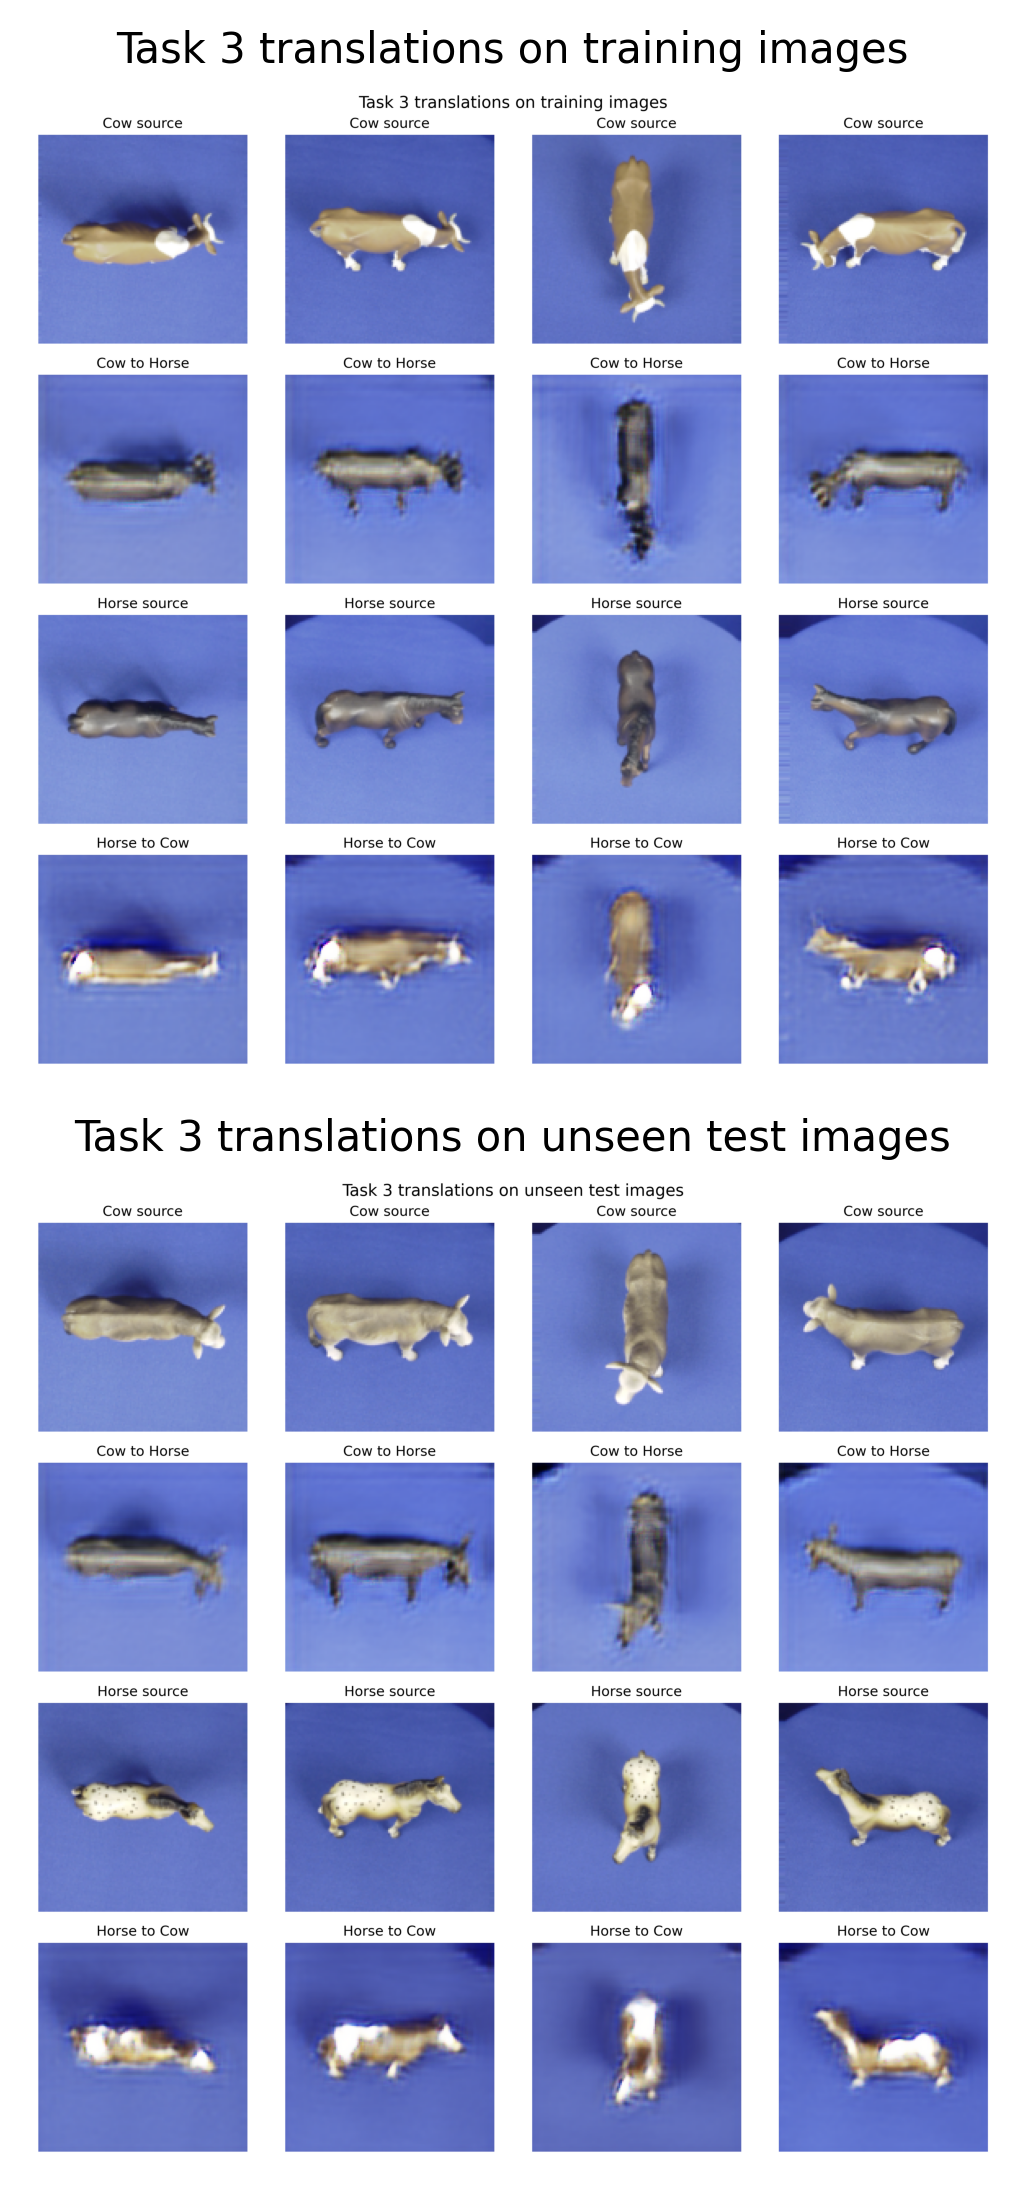
\includegraphics[width=\columnwidth]{generated/figures/task3_overview.png}
\caption{Task 3 qualitative results on training images and unseen test images.}
\label{fig:task3overview}
\end{figure}

\section{Discussion and Conclusion}\label{sec:conclusion}
Two conclusions are the most important. First, stable classification on this dataset requires a from-scratch compact CNN together with a horse-sensitive loss weight and multi-seed ensembling. Second, GAN augmentation becomes useful only after manual curation and asymmetric use. In other words, the best final system is not the most complex one; it is the one that directly corrects the weakest class with carefully selected synthetic examples.

The pretrained-discriminator attempt is also informative. Even though it looked attractive in theory, it produced visually failed horse generations and was therefore rejected. This reinforces the broader result of the project: on a tiny single-instance dataset, engineering choices must be judged by whether they improve the final decision boundary, not only by whether they sound stronger in principle.

\bibliographystyle{IEEEtran}
\bibliography{refs}

\end{document}
